% inspired from http://tex.stackexchange.com/questions/268128/how-to-nicely-place-two-heaps-next-to-each-other
\documentclass{article}

\usepackage{tikz}
\usepackage{array}
\usetikzlibrary{shapes.multipart}

\tikzset{
  heap/.style={
    every node/.style={circle, draw, fill=blue!20},
    level 1/.style={sibling distance=35mm},
    level 2/.style={sibling distance=20mm},
    level 3/.style={sibling distance=9mm}
  }
}

\begin{document}

% Exemple de tas max

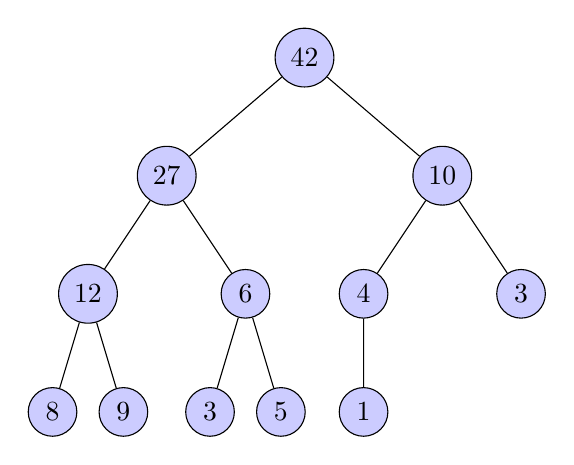
\begin{tikzpicture}[heap]
  \node {42}
  child{node{27}
    child{
    	node{12}
    		child{node{8}}
    		child{node{9}}}
    	child{node{6}
    		child{node{3}}
    		child{node{5}}}}
  child{node{10}
  	child{node{4}
  		child{node{1}}}
  	child{node{3}}}
  ;
\end{tikzpicture}

\vspace{1cm}

% Tableau représentatif du tas

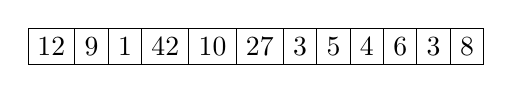
\begin{tikzpicture}
\node[rectangle split, rectangle split horizontal, rectangle split parts = 12, draw]
{
	\nodepart{one}12
	\nodepart{two}9
	\nodepart{three}1
	\nodepart{four}42
	\nodepart{five}10
	\nodepart{six}27
	\nodepart{seven}3
	\nodepart{eight}5
	\nodepart{nine}4
	\nodepart{ten}6
	\nodepart{eleven}3
	\nodepart{twelve}8
};
\end{tikzpicture}

\end{document}